\documentclass[10pt]{article}

%Math
\usepackage{amsmath}
\usepackage{amsfonts}
\usepackage{amssymb}
\usepackage{amsthm}
\usepackage{ulem}
\usepackage{stmaryrd} %f\UTF{00FC}r Blitz!

%Definitionen / Sätze
\usepackage{thmbox}
\newtheorem[M]{definition}{Def.}
\newtheorem[M]{satz}{Satz}
\numberwithin{equation}{section}


%PageStyle
\usepackage[ngerman]{babel} % deutsche Silbentrennung
\usepackage[utf8]{inputenc} 
\usepackage{fancyhdr, graphicx}
\usepackage[scaled=0.92]{helvet}
\usepackage{enumitem}
\usepackage{parskip}
\usepackage[a4paper,top=2cm]{geometry}
\setlength{\textwidth}{17cm}
\setlength{\oddsidemargin}{-0.5cm}



%My Commands
\newcommand{\RN}{\mathbb{R}} %Real Number
\newcommand{\NN}{\mathbb{N}} %Natural Number
\newcommand{\QN}{\mathbb{Q}} %Rational Number
\newcommand{\ZN}{\mathbb{Z}} %ganze Zahlen
\newcommand{\CN}{\mathbb{C}}
\newcommand{\PN}{\mathbb{P}}
\newcommand{\EN}{\mathbb{E}}
\newcommand{\Bold}[1]{\textbf{#1}} %Boldface
\newcommand{\Kursiv}[1]{\textit{#1}} %Italic
\newcommand{\T}[1]{\text{#1}} %Textmode
\newcommand{\Nicht}[1]{\T{\sout{$ #1 $}}} %Streicht Shit durch

%Arrows
\newcommand{\lra}{\leftrightarrow} 
\newcommand{\ra}{\rightarrow}
\newcommand{\la}{\leftarrow}
\newcommand{\lral}{\longleftrightarrow}
\newcommand{\ral}{\longrightarrow}
\newcommand{\lal}{\longleftarrow}
\newcommand{\Lra}{\Leftrightarrow}
\newcommand{\Ra}{\Rightarrow}
\newcommand{\La}{\Leftarrow}
\newcommand{\Lral}{\Longleftrightarrow}
\newcommand{\Ral}{\Longrightarrow}
\newcommand{\Lal}{\Longleftarrow}

% Code listenings
\usepackage{color}
\usepackage{xcolor}
\usepackage{listings}
\usepackage{caption}
\DeclareCaptionFont{white}{\color{white}}
\DeclareCaptionFormat{listing}{\colorbox{gray}{\parbox{\textwidth}{#1#2#3}}}
\captionsetup[lstlisting]{format=listing,labelfont=white,textfont=white}
\lstdefinestyle{JavaStyle}{
 language=Java,
 basicstyle=\footnotesize\ttfamily, % Standardschrift
 numbers=left,               % Ort der Zeilennummern
 numberstyle=\tiny,          % Stil der Zeilennummern
 stepnumber=5,              % Abstand zwischen den Zeilennummern
 numbersep=5pt,              % Abstand der Nummern zum Text
 tabsize=2,                  % Groesse von Tabs
 extendedchars=true,         %
 breaklines=true,            % Zeilen werden Umgebrochen
 frame=b,         
 %commentstyle=\itshape\color{LightLime}, Was isch das? O_o
 %keywordstyle=\bfseries\color{DarkPurple}, und das O_o
 basicstyle=\footnotesize\ttfamily,
 stringstyle=\color[RGB]{42,0,255}\ttfamily, % Farbe der String
 keywordstyle=\color[RGB]{127,0,85}\ttfamily, % Farbe der Keywords
 commentstyle=\color[RGB]{63,127,95}\ttfamily, % Farbe des Kommentars
 showspaces=false,           % Leerzeichen anzeigen ?
 showtabs=false,             % Tabs anzeigen ?
 xleftmargin=17pt,
 framexleftmargin=17pt,
 framexrightmargin=5pt,
 framexbottommargin=4pt,
 showstringspaces=false      % Leerzeichen in Strings anzeigen ?        
}

%Config
\renewcommand{\headrulewidth}{0pt}
\setlength{\headheight}{15.2pt}

%Metadata
\fancyfoot[C]{If you use this documentation for a exam, you should offer a beer to the authors!}
\title{
	\vspace{5cm}
	Wahrscheinlichkeiten und Statistik
}
\author{Jan Fässler}
\date{5. Semester (HS 2013)}


% hier beginnt das Dokument
\begin{document}

% Titelbild
\maketitle
\thispagestyle{fancy}
\newpage

% Inhaltsverzeichnis
\pagenumbering{Roman}
\tableofcontents	  	


\newpage
\setcounter{page}{1}
\pagenumbering{arabic}

% Inhalt Start

\section{Lapdance \& Kombinatorik}

\subsection{Zufallsexperimente \& Wahrscheinlichkeiten}

\begin{definition}[Zufallsexperiment]
Ein Experiment, welches beliebig oft wiederholt werden kann und bei jeder Durchführung ein Ergebnis aus einer bestimmten Menge von möglichen Ergebnissen annimmt.
\end{definition}

\begin{definition}[Ergebnismenge $\Omega$]
Ein Experiment, welches beliebig oft wiederholt werden Mögliche Ergebnisse eines Zufallsexperiments.
\end{definition}

\begin{definition}[Ergebnis]
Aussage, die bei der Durchführung des Experimentes entweder wahr oder falsch ist, je nachdem welches Ergebnis eingetreten ist.
\end{definition}
Jedes Ereignis kann als Teilmenge von Ergebnissen interpretiert werden. \\
\\
Die einzelnen Ergebnisse selber können ebenfalls als Ereignisse betrachtet werden: \\
Zu einem Ergebnis $\omega \in \Omega$ gehört das sogenannte \textbf{Elementarereignis} $E = \{\Omega\}$.

\textbf{Beispiel:  Wurf eines Würfels} \\
Ergebnismenge: $\Omega=\{1,2,3,4,5,6\}$ \\
Beispiel für ein Ereignis:\\
E : \"{}Die augenzahl ist gerade\"{} \\
$E=\{2,4,6\}$ \\

\begin{definition}[Wahrscheinlichkeit]
Mass für die relative Häufigkeit mit der das Ereignis bei wiederholten Durchführung des Experimentes eintritt.
\end{definition}

\subsection{Laplace-Experiment}
\begin{definition}[Laplace-Experiment]
Ein Zufallsexperiment mit $n$ verschiedenen möglichen Ergebnissen, die alle dieselbe Wahrscheinlichkeit, alse $\frac{1}{n}$ haben.
\end{definition}

Die Wahrscheinlichkeit eines Ereignisses $E \subseteq\Omega$ wird für diesen Fall folgendermassen definiert:
\begin{equation}
  P(E)=\frac{|E|}{|\Omega|}=\frac{\text{Anzahl günstige Ergebnisse}}{\text{Anzahl aller Ergebnisse}}
\end{equation}
Dieses mathematische Modell für ein Laplace-Experiment, bestehend aus der Menge $\Omega$ mit der Funktion $P$ nennt man einen \textbf{Laplace-Raum}. Dieses $P$ heisst auch \textbf{Gleichverteilung}. \\
\\
\textbf{Beispiel:  Wurf eines Würfels} \\
Wie gross ist die Wahrscheinlichkeit für eineAugenzahl grösser als 4? \\
$E=\{5,6\}$ \\
\\
$P(E)=\frac{2}{6}=\frac{1}{3} \approx 33.33\%$ \\
\\
Im Laplace-Raum sind für Mengen $M$ die Anzahl der Elemente, $|M|$, zu bestimmen. Die \textbf{Kombinatorik} liefert systematische Abzählverfahren.

\subsection{Kombinatorik}

\subsubsection{Produkte}
\begin{definition}[Produktregel]
Wenn es bei einem mehrstufigen Auswahlprozess für das 1. Objekt $n_1$ Möglichkeiten, für das 2. Objekt $n_2$ Möglichkeiten, \dots , und für das $k$-te Objekt $n_k$ Möglichkeiten gibt, dann gibt es für den gesamten Auswahlprozess $n_1*n_2* \dots * n_k$ Möglichkeiten.
\end{definition}
\begin{center}
	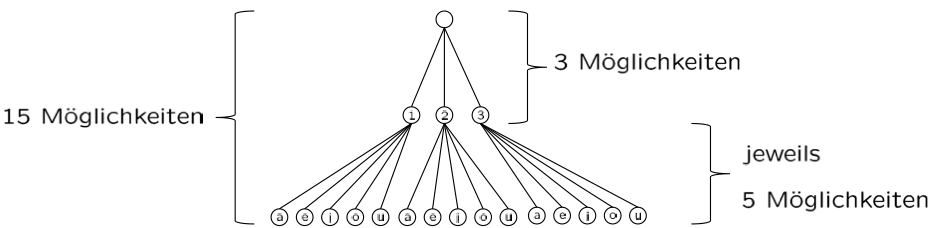
\includegraphics[scale=0.4]{produktregel.png}
\end{center}

\subsubsection{Summen}
\begin{definition}[Summenregel]
Wenn es $n_1$ Objekte mit Eigenschaft 1, $n_2$ Objekte mit Eigenschaft 2, \dots, $n_k$ Objekte mit Eigenschaft $k$ gibt, und kein Objekt zwei der Eigenschaften gleichzeitig besitzt, dann gibt es insgesamt $n_1+n_2+$ \dots $+n_k$ Objekte die eine der Eigenschaft besitzen.
\end{definition}
Beispiel: Eine Meitwagenfirma hat 5 Kleinwagen, 3 Mittelklassewagen und 2 Oberklassewagen. Da kein Auto in mehreren Kategorien sein kann, hat die Firma insgesamt $5+3+2=10$ Wagen.

\subsubsection{Fakultät}
Wir ziehen $n$ mal ohne Zurücklegen mit Beachtung der Reihenfolge aus einer Urne mit $n$ Kugeln. Dan gibt es $n*(n-1)*$ \dots $*2*1$ Möglichkeiten.
\begin{definition}[Fakultät]
Es sei $n \in \NN$. Dann Heisst $n!=n*(n-1)*$ \dots $*2*1$ Fakultät von $n$. Zudem ist $0! := 1$. 
\end{definition}

Es gilt $n! \sim \sqrt{2*\pi*n}*(\frac{n}{e})^n$

\subsubsection{Binominalkoeffizient}
Wir ziehen $k$ mal aus einer Menge von $n$ Zahlen ohne Zurücklegen und ohne Beachtung der Reihenfolge. Es gibt also $\frac{n!}{(n-k)!*k!}$ Möglichkeiten.
\begin{definition}[Binominalkoeffizient]
Es sei $0 \leq k \leq n$. \\
Dann ist der Binominalkoeffizient $\binom{n}{k}$ definiert als $\frac{n!}{(n-k)!*k!}$. \\
Für $k > n$ ist $\binom{n}{k} := 0$.
\end{definition}
$\binom{n}{k}$ gibt also die Anzahl aller $k$-elementigen Teilmengen einer $n$-elementigen Menge an.

\subsection{Urnenmodel}
Viele Abzählprobleme lassen sich auf das sogenannte Urnenmodell zurückführen. Gegeben ist eine Urne mit $n$ unterschiedlichen Kugeln. Wir ziehen $k$ Kugeln aus den $n$ Kugeln. Auf wieviele Arten geht diesm wenn unterschieden wird nach "`Zurücklegen"' oder "`nicht zurücklegen"' und "`geordnet"' oder "`keine Reihenfolge"'? \\
\\
\begin{description}
	\item[k:] Anzahl Ziehungen
	\item[n:] Anzahl Elemente
\end{description}
\begin{tabular}{l|l|l}
 &zur\"{u}cklegen&nicht zur\"{u}cklegen\\\hline
 geordnet&$n^k$&$n!$ oder $\frac{n!}{(n-k)!}$\\\hline
 ungeordnet&$\binom{k+n-1}{k}$&$\binom{n}{k}=\frac{n!}{k!(n-k)!}$
\end{tabular}\\

\newpage
\section{Allgemeine Wahrscheinlichkeiten}
\subsection{Einleitung}
\begin{definition}[Wahrscheinlichkeit]
Eien Wahrscheinlichkeit $P: 2^{\Omega} \rightarrow [0,1]$ erfüllt:
\begin{description}
	\item[(1)] $P(\Omega) = 1$
	\item[(2)] Für endlich oder abzählbar viele parweise disjunktive Ereignisse $E_1,E_2,E_3, $\dots gilt: \\
	 $P(E_1 \cup E_2 \cup E_3 \cup$ \dots $) = P(E_1) + P(E_2) + P(E_3) + $ \dots 
\end{description}
\end{definition}
\begin{satz}
Es sei $P$ eine Wahrscheinlichkeit auf $\Omega$. Dan gilt:
\begin{description}
	\item[(1)] $\forall E \subseteq \Omega : P(E^c)=1-O(E)$
	\item[(2)] $P(0) = 0$
	\item[(3)] $\forall E_1, E_2 \subseteq \Omega : P(E_1\cup E_2) = P(E_1) + P(E_2) - P(E_1 \cap E_2)$
	\item[(4)] Für eine endliche oder abzählbare Menge $E=\{e_1,e_2,$ \dots $\}$ gilt $P(E) = P(\{e_1\}) + P(\{e_2\}) +$ \dots
\end{description}
\end{satz}
Die Wahrscheinlichkeitsverteilung $P$ durch die Angabe der Wahrscheinlichkeiten ist für die Elementarereignisse festgelegt, falls $\Omega$ endlich oder abzählbar ist.
\begin{definition}[Zähldichte (Z-Dichte)]
Die Funktion $f_P : \Omega \rightarrow [0,1]$ mit $f_P(w)=P(\{w\})$ heisst Zähldichte von P.
 \end{definition}
 In diesem Fall gilt also $P(E)=\sum_{e \in E} f_P(e)$, insbesondere $P(E)=\sum_{e \in \Omega} f_P(e)=1$
 
\subsection{bedingte Wahrscheinlichkeit}
Würfeln mit einem normalen Würfel: $\Omega = \{1,2,3,4,5,6\}$, $P=$ Gleichverteilung. Wie hoch ist die Wahrscheinlichkeit  für $A=\{2,3\}$, wenn ich weiss, dass eine ungerade Zahl gewürfelt worden ist? \\
Es verbleibt noch die eingeschränkte Ergebnismenge $B=\{1,3,5\}$. \\
Es sind also nur noch $|B|=3$ Ergebnisse möglich. \\
Davon sind $|A \cap B|=1$ Ergebnisse günstig. \\
Die gesuchte Wahrscheinlichkeit ist somit $\frac{|A \cap B|}{|B|} = \frac{1}{3}$.
\begin{definition}[bedingte Wahrscheinlichkeit]
Es sei $\Omega$ eine nichtleere endliche Menge und $P$ eine Wahrscheinlichkeitsverteilung auf $\Omega$. Ferner sei $B \subseteq \Omega$ mit $P(B) > 0$. \\
Dann heisst $P(A|B) := \frac{P(A \cap B)}{P(B)}$ (elementare) bedingte Wahrscheibnlichkeit von A unter B.
\end{definition} 
\begin{definition}[Formel von Bayes]
Es sei $\Omega$ eine nichtleere endliche Menge und $P$ eine Wahrscheinlichkeitsverteilung auf $\Omega$. Ferner seien $A,B \subseteq \Omega$ mit $P(A) > 0$ und $P(B) > 0$. \\
Dann gilt $P(A|B)=\frac{P(A)}{P(B)} * P(B | A)$.
\end{definition} 
\begin{definition}[totele Wahrscheinlichkeit]
Es sei $\Omega$ eine nichtleere endliche Menge und $P$ eine Wahrscheinlichkeitsverteilung auf $\Omega$. Ferner seien $B_i(i \in I)$ eine Zerlegung von $\Omega$ (d.h. die $B_i$ sind paarweise disjunkt und $\Omega=U_{i \in I} B_i$) mit $P(B_i) > 0$. \\
Dann gilt $P(A) = \sum_{i \in I} P(A | B_i) * P(B_i)$
\end{definition} 
\begin{definition}[positive prädiktive Wert]
Für $0 < P(A) < 1$ gilt mit $\Omega = A \cup A^c$ insbesondere: \\
$P(A | B) = \frac{P(A)*P(A | B)}{P(B | A) * P(A) + P(B | A^c) * P(A^c)}$
\end{definition} 

\subsection{stochastische Unabhängigkeit}
\begin{definition}[stochastisch unabhängig]
Es sei $P$ eine Wahrscheinlichkeitsverteilung auf $\Omega$. \\
Zwei Ereignisse $A,B \subseteq \Omega$ heissen stochastisch unabhängig, falls $P(A \cap B) = P(A) * P(B)$. \\
Im Falle $P(B) \neq 0$ ist dies äquivalent zu $\underbrace{P(A|B)}_{\frac{P(A \cap B)}{P(B)}}=P(A)$.
\end{definition} 

\subsection{Mehrstufige Zufallsexperimente}
Ein $n$-stufiger Versuch mit Ergebnismenge $\Omega_i$ für den $i$-ten Versuch wird meist wie folgt modelliert:
\begin{description}
	\item[(1)] Man legt die Dichte $f_1(\omega_1)$ auf $\Omega_1$ für den ersten Versuch fest.
	\item[(2)] Man legt die Dichte $f_2(\omega_2 | \omega_1)$ auf $\Omega_2$ für den zweiten Versuch in Abhängigkeit vom Ergebnis $\omega_1$ des ersten Versuchs fest.
	\item[(3)] Man legt die Dichte $f_3(\omega_3 | \omega_1, \omega_1)$ auf $\Omega_3$ für den dritten Versuch in Abhängigkeit der Ergebnisse ($\omega_1, \omega_2$) der ersten beiden Versuche fest.
	\item \dots
	\item[(n)] Man legt die Dichte $f_n( \omega_n | \omega_1,$, \dots,$\omega_{n-1}$) auf $\Omega_n$ für den $n$-ten Versuch in Abhängigkeit der Ergebnisse ($\omega_1$, \dots, $\omega_{n-1}$) der ersten $n$ Versuche fest. 
	\item[(n+1)] Die resultierende Dichte auf $\Omega_1$ x $\Omega_2$ x \dots x $\Omega_n$ ist dann $f(\omega_1$, \dots, $\omega_n) = f_1(\omega_1) * f_2(\omega_2 | \omega_1) * $ \dots $ * f_n(\omega_n | \omega_1$, \dots, $\omega_{n-1}$).
\end{description}
Wenn die Versuche nicht voneinander abhängen, dann modelliert man die Versuche einzeln, mit Dichten $f_i(\omega_i)$ auf $\Omega_i$, und erhält als resultierende Dichte $f(\omega_1,$ \dots, $\omega_n)=f1(\omega_1) *$ \dots $* f_n(\omega_n)$. \\
\begin{center}
	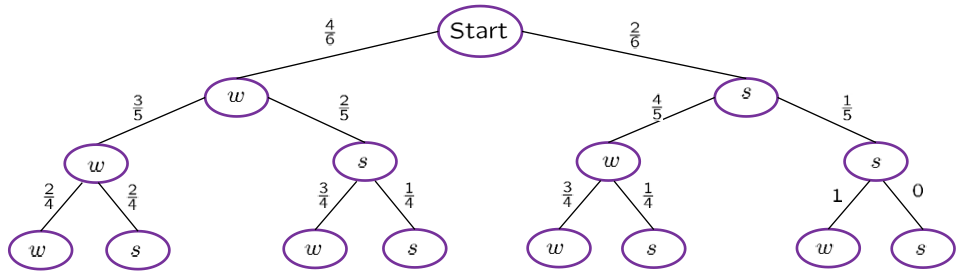
\includegraphics[scale=0.4]{mehrstuffigeW.png}
\end{center}

\newpage
\section{diskrete Zufallsvariablen}
\subsection{Zufallsvariablen}
Eine Zufallsvariable ist eine normale mathematische Funktion. Da bei jeder Durchführung des Zufallsexperiments ein zufälliges Ergebnis $\omega$ eintritt, ist auch der zugehörige Wert $X(\omega)$ nicht vorhersagbar.
\begin{definition}[Zufallsvariable]
Eine Zufallsvariable $X$ über $\Omega$ ist eine Abbildung ovn $\Omega$ in einere Menge $X$. Im Folgenden wird stehts $X \subseteq \RN$ sein. Dan sagt man auch reellwertige Zufallsvariable.
\end{definition}
$X$ induziert eine Wahrscheinlichkeitsverteilung $P^X$ auf $X$ durch $P^X(A)=P(X^{-1}(A))$, wobei $X^{-1}(A)$ das Urbild von A bezeichnet. \\
$P^X$ heisst Verteilung von X oder bildmass von X unter P.

\subsection{Verteilungsfunktion}
\begin{definition}[Verteilungsfunktion]
Es sei $X : \Omega \rightarrow X$ eine Zufallsvariable, wobei $X \in \RN$ eine endliche oder abzählbare Menge ist. Zudem sei $f$ die Zähldichte von $X$. \\
Dann heisst $F(x)=P(X \leq x) = \sum_{t \in X:t \leq x} f(t)$ Verteilungsfunktion von X.
\end{definition}
\begin{center}
	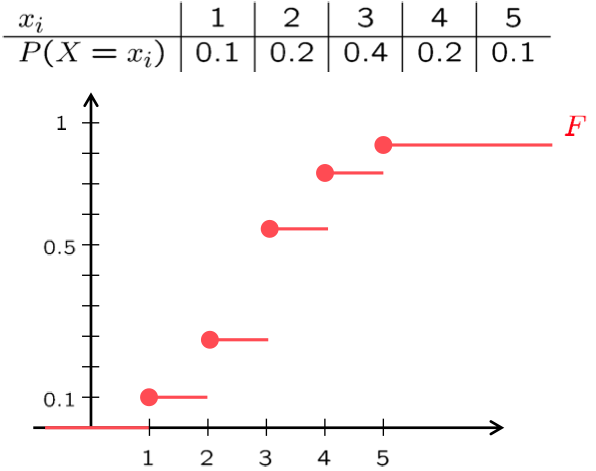
\includegraphics[scale=0.3]{verteilungsfunktion.png}
\end{center}

\subsection{Erwartungswert}
\begin{definition}[Erwartungswert]
Es sei $X : \Omega \rightarrow X$ eine Zufallsvariable, wobei $X \subset \RN$ eine endliche oder abzählbare Menge ist. Zudem sei $f$ die Zähldichte von $X$. \\
Dann heisst $E(X)=\sum_{x \in X} x * f(x)=\sum_{x \in X} x * P(X = x)$ Erwartungswert von X.
\end{definition}

\subsection{Varianz und Standardabweichung}
\begin{definition}[Varianz]
Es sei $X : \Omega \rightarrow X$ eine Zufallsvariable, wobei $X \subset \RN$ eine endliche oder abzählbare Menge ist. Zudem sei $f$ die Zähldichte von $X$ und $\mu$ der Erwartungswert von $X$. \\
Dann heisst $V(X) = \sum_{x \in X} (x - \mu)^2 * f(x) = \sum_{x \in X} (x - \mu)^2 * P(X=x)$ Varianz von $X$.
\end{definition}
Durch das Quadrieren heben sich Abweichung nach unten und nach oben nicht auf, zudem werden grössere Abweichungen stärker gewichtet. \\
\begin{definition}[Standardabweichung]
$\sigma(X) = \sqrt{V(X)}$ heisst Standardabweichung von $X$.\\
\end{definition}
Die Varianz und die Standardabweichung sind MAsse für die Streuung der Zufallsvariable um den Erwartungswert. \\
Zur Berechnung der Varianz ist es manchmal einfacher, folgende Formel zu verwenden:
\begin{satz}
Es sei $X : \Omega \rightarrow X$ eine Zufallsvariable, wobei $X \subset \RN$ eine endliche oder abzählbare Menge ist. \\
Dan gilt $V(X) = E(X^2)-E(X)^2$.
\end{satz}

\newpage
\section{diskrete Verteilung}
\begin{tabular}{l l}
	Alle Ereignisse gleich wahrscheinlich & Laplace \\
	\\
	Treffer$(WK p)$, nciht Treffer & $B(p)$ \\
	\\
	Anzahl Treffer $(WK p)$ in $n$ unabhängigen Versuchen & $Bin(n,p)$ \\
	\\
	Versuche bis erster Treffer $(WK p)$ in unabhängigen Versuchen & $Geo(p)$ \\
	\\
	Verteilung für seltene Ereignisse mit im Schnitt $\lambda$ Ereignissen pro Zeit/Ort-Einheit & $Poi(\lambda)$ \\
\end{tabular}

\subsection{Bernoulli-Verteilung}
\begin{definition}[Bernoulli-Verteilung]
Die Verteilung einer Zufallsvariable X, die nur zwei Werte 0 (Treffer) oder 1 (kein Treffer) annehmen kann, wobei $p$ die Wahrscheinlichkeit für 1 bezeichent, heisst Bernoulli-verteilt mit Parameter $p$. \\
\end{definition}
Schreibweise: $X \sim B(p)$ \\
Dichte von $X : f(0) = 1 - p$, $f(1) = p$ \\
\\
$E(X) = p$ \\
$V(X) = p*(1-p)$ \\

\subsection{Binomial-Verteilung}
\begin{definition}[Binomial-Verteilung]
Die Verteilung einer Zufallsvariable X, die die Anzahl an Treffern bei der $n$-maligen unabhängigen Durchführung eines Experiments mit zwei Ausgängen, Treffer oder kein Treffer, wobei $p$ die Wahrscheinlichkeit für Treffer bezeichnet, heisst Binomial-verteilt mit Parametern $n,p$. \\
\end{definition}
Schreibweise: $X \sim Bin(n,p)$ \\
Dichte von $X : f(k) = \binom{n}{k} * p^k * (1-p)^{n-k}$, $k=0,1,$ \dots, $n$ \\
\\
$E(X) = n*p$ \\
$V(X) = n*p*(1-p)$ \\

\subsection{geometirsche-Verteilung}
\begin{definition}[geometischre-Verteilung]
Die Verteilung einer Zufallsvariable X, die die Anzahl der Versuche bis zum ersten Treffer bei der $n$-maligen unabhängigen Durchführung eines Experiments mit zwei Ausgängen, Treffer und kein Treffer, wobei $p$ die Wahrscheinlichkeit für Treffer bezeichnet, heisst geometrisch verteilt mit Parameter $p$. \\
\end{definition}
Schreibweise: $X \sim Geo(n,p)$ \\
Dichte von $X : f(k) = (1-p)^{k-1}*p$, $k=0,1,$ \dots, $n$ \\
$X=k$ bedeutet, dass die ersten $k-1$ Versuche jeweils kein Treffer waren. und der $k$-te Versuch ein Treffer war.
\\
$E(X) = \frac{1}{p}$ \\
$V(X) = \frac{1-p}{p^2}$ \\

\subsection{Poisson-Verteilung}
\begin{definition}[Poisson-Verteilung]
Die Poisson-Verteilung kommt bei Zufallsvariablen zum Einsatz, welche die Anzahl Ereignisse einer bestimmten Art in einer Zeit- und/oder Ort-Intervall beschreiben. Falls im Mittel $\lambda$-Ereignisse auftreten, dann ist X Poisson verteilt mit Parameter $\lambda$. \\
\end{definition}
Schreibweise: $X \sim Poi(\lambda)$ \\
Dichte von $X : f(k) =\frac{\lambda^k}{k!}*e^{-\lambda}$, $k=0,1,$ \dots, $n$ \\
$X=k$ bedeutet, dass die ersten $k-1$ Versuche jeweils kein Treffer waren. und der $k$-te Versuch ein Treffer war.
\\
$E(X) = \lambda$ \\
$V(X) = \lambda$ \\

\subsection{Eigenschaften}
\begin{satz}
Es seien $X,Y$ Zufallsvariablen und $a,c \in \RN$.
Dan gilt:
\begin{itemize}
	\item $E(X + Y) = E(X) + E(Y)$ 
	\item $E(a * X) = a * E(X)$
	\item $E(X + c) = E(X) + c$ 
	\item $V(X + c) = V(X)$
	\item $V(a * X) = a^2* V(X)$
	\item $E(g(X)) = \sum_{x} g(x) * P(X=x)$ für alle Funktionen g: $\RN \rightarrow \RN$
	\item $E(g(X)) \neq g(E(X))$.
\end{itemize}
\end{satz}

% Inhalt Ende 
\end{document} 